%% LyX 2.3.4.2 created this file.  For more info, see http://www.lyx.org/.
%% Do not edit unless you really know what you are doing.
\documentclass[twocolumn,english,final,3p,times, english]{elsarticle}
\usepackage[utf8]{inputenc}
\usepackage{color}
\usepackage{babel}
\usepackage{array}
\usepackage{booktabs}
\usepackage{multirow}
\usepackage{amsmath}
\usepackage{amsthm}
\usepackage{amssymb}
\usepackage{graphicx}
\usepackage[unicode=true,
 bookmarks=false,
 breaklinks=false,pdfborder={0 0 1},backref=section,colorlinks=true]
 {hyperref}
\hypersetup{
 linkcolor=black,filecolor=black,urlcolor=cyan}

\makeatletter

%%%%%%%%%%%%%%%%%%%%%%%%%%%%%% LyX specific LaTeX commands.
%% Because html converters don't know tabularnewline
\providecommand{\tabularnewline}{\\}

%%%%%%%%%%%%%%%%%%%%%%%%%%%%%% User specified LaTeX commands.
%%
%% Copyright 2007, 2008, 2009 Elsevier Ltd
%%
%% This file is part of the 'Elsarticle Bundle'.
%% ---------------------------------------------
%%
%% It may be distributed under the conditions of the LaTeX Project Public
%% License, either version 1.2 of this license or (at your option) any
%% later version.  The latest version of this license is in
%%    http://www.latex-project.org/lppl.txt
%% and version 1.2 or later is part of all distributions of LaTeX
%% version 1999/12/01 or later.
%%
%% The list of all files belonging to the 'Elsarticle Bundle' is
%% given in the file `manifest.txt'.
%%

%% Template article for Elsevier's document class `elsarticle'
%% with numbered style bibliographic references
%% SP 2008/03/01
%%
%%
%%
%% $Id: elsarticle-template-num.tex 4 2009-10-24 08:22:58Z rishi $
%%
%%
%%\documentclass[preprint,12pt,3p]{elsarticle}

%% Use the option review to obtain double line spacing
%%\documentclass[preprint,review,12pt]{elsarticle}

%% Use the options 1p,twocolumn; 3p; 3p,twocolumn; 5p; or 5p,twocolumn
%% for a journal layout:
%% \documentclass[final,1p,times]{elsarticle}
%% \documentclass[final,1p,times,twocolumn]{elsarticle}
%% \documentclass[final,3p,times]{elsarticle}
%% \documentclass[final,5p,times]{elsarticle}
%% \documentclass[final,5p,times,twocolumn]{elsarticle}

%% if you use PostScript figures in your article
%% use the graphics package for simple commands
%% \usepackage{graphics}
%% or use the graphicx package for more complicated commands
%% \usepackage{graphicx}
%% or use the epsfig package if you prefer to use the old commands
%% \usepackage{epsfig}


%% The amssymb package provides various useful mathematical symbols
\usepackage{blindtext}
\usepackage{algorithm}\usepackage{algpseudocode}\usepackage{pifont}\usepackage{algcompatible}\usepackage{comment}\usepackage{layout}\usepackage{amsthm}\usepackage{enumitem}
\usepackage{eso-pic}
\usepackage{float}
%% The amsthm package provides extended theorem environments
%% \usepackage{amsthm}
\renewcommand{\qedsymbol}{$\blacksquare$}

%\usepackage[english]{babel}

\usepackage[justification=centering]{caption}
\usepackage{caption}
\captionsetup{justification=raggedright, singlelinecheck = false}
\captionsetup[table]{labelformat=simple, labelsep=newline}
\captionsetup[figure]{labelformat=simple, labelsep=period}


%% The lineno packages adds line numbers. Start line numbering with
%% \begin{linenumbers}, end it with \end{linenumbers}. Or switch it on
%% for the whole article with \linenumbers after \end{frontmatter}.
%% \usepackage{lineno}

%% natbib.sty is loaded by default. However, natbib options can be
%% provided with \biboptions{...} command. Following options are
%% valid:

%%   round  -  round parentheses are used (default)
%%   square -  square brackets are used   [option]
%%   curly  -  curly braces are used      {option}
%%   angle  -  angle brackets are used    <option>
%%   semicolon  -  multiple citations separated by semi-colon
%%   colon  - same as semicolon, an earlier confusion
%%   comma  -  separated by comma
%%   numbers-  selects numerical citations
%%   super  -  numerical citations as superscripts
%%   sort   -  sorts multiple citations according to order in ref. list
%%   sort&compress   -  like sort, but also compresses numerical citations
%%   compress - compresses without sorting
%%
%% \biboptions{comma,round}

% \biboptions{}
\newtheorem{theorem}{Theorem}\newtheorem{lemma}{Lemma}\newtheorem{definition}{Definition}

\journal{ICT Express}

%\newcommand\AtPagemyUpperRight[1]{\AtPageLowerRight{%
%\put(\LenToUnit{0.8\paperwidth},\LenToUnit{0.9\paperheight}){#1}}}
%\AddToShipoutPictureFG{
%  \AtPagemyUpperRight{{\includegraphics[width=.5cm,keepaspectratio]{logo.png}}}
%}%
%\newcommand\AtPagemyUpperLeft[1]{\AtPageLowerLeft{%
%\put(\LenToUnit{0.85\paperwidth},\LenToUnit{0.9\paperheight}){#1}}}
%\AddToShipoutPictureFG{
%  \AtPagemyUpperLeft{{\includegraphics[width=1.0cm,keepaspectratio]{logo2.jpg}}}
%}%

\makeatother
\def\@author#1{\g@addto@macro\elsauthors{\normalsize%
    \def\baselinestretch{1}%
    \upshape\authorsep#1\unskip\textsuperscript{%
      \ifx\@fnmark\@empty\else\unskip\sep\@fnmark\let\sep=,\fi
      \ifx\@corref\@empty\else\unskip\sep\@corref\let\sep=,\fi
      }%
    \def\authorsep{\unskip,\space}%
    \global\let\@fnmark\@empty
    \global\let\@corref\@empty  %% Added
    \global\let\sep\@empty}%
    \@eadauthor={#1}
}
\makeatother

\begin{document}
\begin{frontmatter}

\title{Towards Detecting Dictionary Based Malicious Domain Names}
%\author{Author’s Full Name 1\corref{cor1}, Author’s Full Name 2, Author’s Full Name 3}

\author{Amir Mukeri \corref{cor1}}

\ead{mukeriamir@gmail.com}

\author{Dwarkoba Gaikwad\corref{cor2}}

\ead{dpgaikwad@aissmscoe.com}

\address{Department of Computer Engineering, AISSMS College of Engineering,
Pune, India}

\cortext[cor1]{Corresponding author}

%\ead{author1@ictexpress.com, author2@ictexpress.com, author2@ictexpress.com}
\begin{abstract}
Domain Generation Algorithms are used by cyber attackers to generate
arbitrary domain names for their Command \& Control servers. These
algorithms are now relying on dictionary wordlist-based domain names.
We present a model based on Bi-Directional Encoder Representation
from Transformer architecture to detect and classify such malicious
domain names. It can help in detecting and blocking rogue domain names.
Proposed model outperforms state-of-the-art alternative approaches
by a significant margin for both dictionary based as well as randomly
generated domain names.
\end{abstract}
%% keywords here, in the form: keyword \sep keyword

\begin{keyword}
Domain Generation Algorithm \sep Domain Name Server \sep Malware
\sep NLP\sep Transformer %% MSC codes here, in the form: \MSC code \sep code
%% or \MSC[2008] code \sep code (2000 is the default)
\end{keyword}
\end{frontmatter}

%%
%% Start line numbering here if you want
%%
% \linenumbers

%% main text


\section{Introduction}

Malware, such as ransomware, must interact with their respective Command
\& Control (C\&C) server once infected.Malwares rely on domain names
produced by the Domain Generation Algorithm (DGA) to communicate with
command and control servers. Attackers register Algorithmically Generated
Domain (AGD) names. Attackers register Algorithmically Generated Domain
(AGD) names. Upon successful contact, the malware either leaks data
to the C\&C server or infects additional machines in the victim's
network. In the event of a ransomware attack, malware encrypts the
victim's data.

Malicious domain names, such as \emph{ocufxskoiegqvv.com}, might be
gibberish. Huge number of lookup messages for such nonsensical domains,
on the other hand, make it harder to discover and block rogue domains.
DGAs now create domain names based on valid dictionary or wordlist
names, such as \emph{scoreadmireluckapplyfitcouple.com}, rather than
random character based names. Domain blacklisting is a common strategy
for preventing such domain names from being contacted. However, this
method can be easily evaded using sophisticated big wordlist based
domain names.

This paper presents the implementation of an AGD detection technique
based on the Bidirectional Encoder Representational from Transformer
(BERT) model. This approach doesn't require feature selection or hyperparameter
tuning of model.

\section{Related Work}

Kührer et al. \citep{kuhrer2014paint} found that public and vendor
provided domain name blacklists contained only 20\% of major domains
from malware families and failed to provide any protection AGD names.
Antonakakis et al. \citep{antonakakis2012throw} suggested clustering
and classification based approach to process the domain names in respective
DGA families. Woodbridge et al. \citep{woodbridge2016predicting}
used Long Short Term Memory (LSTM) architecture to detect the AGD
names, however faced challenges with dictionary or wordlist based
DGA. Yu et al. \citep{yu2017inline}proposed a system for inline AGD
detection at the DNS server using Convolutional Neural Network (CNN)
and LSTM based approach. A hybrid neural network approach comprising
of parallel CNN and attention based Bi-LSTM layers was designed by
Yang et al. \citep{yang2020detecting}. For multiclass classification
they were able to obtain an macro averaging F1 score of 0.7653 with
proposed hybrid architecture. Another similar approach utilizing attention
based mechanism was proposed by Fangali et al. \citep{ren2020dga}
that uses CNN, Bi-LSTM and Attention layer after the embedding layer
to do the detection as well as multiclass classification of various
DGAs. They obtained micro average F1 score of 0.89 and macro average
score of 0.83 on more than 20 real world AGD name list and legitimate
domain name lists including word list based DGAs such as \emph{matsnu}
and \emph{suppobox}.

\section{Methodology}

Starting with basic neural networks, increasingly sophisticated models
such as CNN, RNN, LSTM, Bi-LSTM, Stacked-LSTM, and eventually BERT
were developed. Character level embedding was utilized in all of the
studies.

DNN with 3 dense hidden layers and 128 neurons was utilized, with
the \emph{relu} activation function. \emph{Dropout} was employed after
each dense layer to avoid overfitting. The CNN model was made up of
a SpatialDropout1D layer, one convolution 1D layer, and a max-pooling
layer. Stacked LSTM units are made up of two bi-directional LSTM layers,
each with 64 units.

\subsection{Transformers and Bidirectional Encoder Representations from Transformer(BERT)}

Similar to the human brain, the attention mechanism in artificial
neural networks aids in focusing on more relevant words in a phrase
while determining how much significance to assign to each word. Vaswani
et al. \citep{vaswani2017attention} presented an attention-based
Transformer neural network design. They eliminated the recurrent layers,
which reduced training time and allowed them to use parallel processes.
Encoder and decoder components make up the transformer architecture.
For neural machine translation, source language statement is embedded
and processed by encoder while the target language translation so
far is produced by decoder as one token at a time. Attention mechanism
works by querying a \emph{query} vector against database of \emph{key}
vectors that are mapped to set of \emph{values} (output values so
far) as depicted in equation \ref{eq:AttentionEquation}.

\begin{equation}
Attention(Q,K,V)=softmax(\frac{QK^{T}}{\sqrt{d_{k}}})V\label{eq:AttentionEquation}
\end{equation}

Attention is a scaled dot product that assigns a probability distribution
to keys that are closely matching with the query vector Q. In practice
Transformers employ multi-head attention, which entails numerous projections
utilizing equation \ref{eq:AttentionEquation}.

Devlin et al. \citep{devlin2018bert} in 2018 used transfer learning
to create Bidirectional Encoder Representations from Transformer (BERT).
Transfer learning enables a model trained on one dataset to be used
for a specific downstream task involving a different dataset. It is
based on the Transformer architecture, although it only employs the
Transformer encoder. BERT training is divided into two stages: \emph{Pre-training}
and \emph{Fine-Tuning.}

During the \textbf{pre-training phase}, BERT builds natural language
understanding through unsupervised learning utilizing Masked Language
Modeling (MLM) and Next Sentence Prediction (NSP). MLM is an unsupervised
task in which a random word in a sentence is masked and the model
predicts the probability distribution over output words. BERT employs
a deep bidirectional model for language modeling rather than just
left-to-right or concatenating two model outputs. In the case of NSP,
given a pair of sentences A and B, if B follows A, it is labelled
as \emph{IsNext}; otherwise, it is labelled as \emph{NotNext}. BERT
is trained on the massive Wikipedia and BookCorpus.

During the \textbf{fine-tuning phase}, BERT is trained on task-specific
labelled datasets such as sentiment classification or question-answering
datasets. During this step, the pre-trained model is trained from
start to finish again, and all parameters are fine-tuned for the specific
task. This is a pretty low-cost and less time-consuming activity.

For the problem at the hand, $BERT_{base}$ model with total of 110M
parameters was used. Fine-tuning was done using labelled DGA dataset
as shown in Figure
\begin{figure}
\begin{centering}
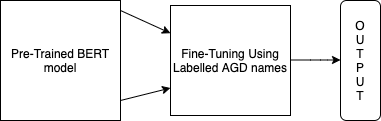
\includegraphics[scale=0.55]{BERT_Training}
\par\end{centering}
\caption{\label{fig:BERT-fine-tuning}Fine tuning of pre-trained BERT model
using labelled dataset}

\end{figure}


\section{Experimental Results and Discussion}

\subsection{Dataset}

For the experimental investigation, real-world domain names generated
by domain generation algorithms were utilized \citep{zago2020umudga}.
The dataset contained 110,000 genuine domain names as well as about
10000 domain names created by various DGAs. The dataset was divided
into two parts: training and testing, with a 70:30 mix of randomly
selected samples. Character level encoding was used to encode the
entire dataset. The task was divided into two parts: DGA detection
and DGA classification.

\subsection{DGA Detection}

In detection task the objective is to design a classifier to successfully
detect whether a domain name is legitimate or malicious. Starting
with simple DNN architecture other architectures were designed and
tested. Results from these experiments are summarized in Table \ref{tab:Results-Detection}
\begin{table*}
\caption{\label{tab:Results-Detection}Detection results on test data. BERT
outperforms all the other models. P:Precision, R:Recall.}

\centering{}%
\begin{tabular}{cccccccccccc}
\toprule
\multirow{2}{*}{Domain Type} & \multicolumn{2}{c}{DNN} & \multicolumn{2}{c}{CNN} & \multicolumn{2}{c}{RNN} & \multicolumn{2}{c}{Bi-LSTM} & \multicolumn{2}{c}{BERT} & Support\tabularnewline
\cmidrule{2-12} \cmidrule{3-12} \cmidrule{4-12} \cmidrule{5-12} \cmidrule{6-12} \cmidrule{7-12} \cmidrule{8-12} \cmidrule{9-12} \cmidrule{10-12} \cmidrule{11-12} \cmidrule{12-12}
 & P & \multicolumn{1}{c}{R} & P & R & P & \multicolumn{1}{c}{R} & P & R & P & R & \tabularnewline
\midrule
legit & 0.97 & 0.97 & \multicolumn{1}{c}{0.99} & 0.98 & 0.98 & 0.95 & 0.98 & 0.99 & 0.99 & 0.99 & 56873\tabularnewline
\midrule
AGD & 0.95 & 0.96 & 0.96 & 0.98 & 0.91 & 0.96 & 0.98 & 0.97 & 0.99 & 0.99 & 32992\tabularnewline
\midrule
\emph{macro avg} & 0.96 & 0.97 & 0.97 & 0.98 & 0.94 & 0.95 & 0.98 & 0.98 & \textbf{0.99} & \textbf{0.99} & 89865\tabularnewline
\midrule
\emph{weighted avg} & 0.97 & 0.97 & 0.98 & 0.98 & 0.95 & 0.95 & 0.98 & 0.98 & \textbf{0.99} & \textbf{0.99} & 89865\tabularnewline
\bottomrule
\end{tabular}
\end{table*}
 BERT was proven to be the best performing model, with a precision,
recall, and accuracy score of 0.99. The proposed BERT model improves
on recent findings published by Yang et al. \citep{yang2020detecting}
and Fangali et al. \citep{ren2020dga} by more than 9 points in absolute
terms.

Furthermore, as seen in Figure \ref{fig:BERT-detection-confidence},
the model is highly confident in its classification of test domain
names.
\begin{figure}
\begin{centering}
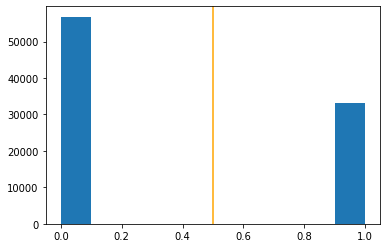
\includegraphics[scale=0.45]{BERT_Binary_Confidence}
\par\end{centering}
\centering{}\caption{\label{fig:BERT-detection-confidence}BERT model AGD(1) vs Legitimate(0)
domain name detection confidence. Value of 0.5 was used as threshold,
shown as orange line.}
\end{figure}


\subsection{DGA Classification}

For this task, the problem was defined as classification task in which
an output label may belong to either legit or one of 19 DGA classes.
Results from test data are shown in Table \ref{tab:Results-on-test}.
The classification efficacy of the BERT model is highest for random
and dictionary-based algorithms like \emph{gozi, matsnu,} and \emph{suppobox}.
BERT based classifier outperforms other methods from recent works
in \citep{yang2020detecting} and \citep{ren2020dga} for both dictionary
based and random DGAs.

\begin{table*}
\caption{\label{tab:Results-on-test}Results on test data. Dictionary based
DGAs are in bold. P:Precision, R:Recall}

\centering{}%
\begin{tabular}{cccccccccccc}
\toprule
\multirow{2}{*}{Domain Type} & \multicolumn{2}{c}{DNN} & \multicolumn{2}{c}{CNN} & \multicolumn{2}{c}{RNN} & \multicolumn{2}{c}{Bi-LSTM} & \multicolumn{2}{c}{BERT} & Support\tabularnewline
\cmidrule{2-12} \cmidrule{3-12} \cmidrule{4-12} \cmidrule{5-12} \cmidrule{6-12} \cmidrule{7-12} \cmidrule{8-12} \cmidrule{9-12} \cmidrule{10-12} \cmidrule{11-12} \cmidrule{12-12}
 & P & R & P & R & P & R & P & R & P & R & \tabularnewline
\midrule
alureon & 0.86 & 0.94 & 0.68 & 0.88 & 0.88 & 0.97 & 0.90 & 0.98 & 0.87 & 0.95 & 2987\tabularnewline
\midrule
banjori & 1.00 & 1.00 & 1.00 & 1.00 & 1.00 & 1.00 & 1.00 & 1.00 & 1.00 & 1.00 & 2958\tabularnewline
\midrule
cryptolocker & 0.68 & 0.73 & 0.66 & 0.59 & 0.75 & 0.68 & 0.72 & 0.77 & 0.70 & 0.73 & 3007\tabularnewline
\midrule
dyre & 1.00 & 1.00 & 1.00 & 1.00 & 1.00 & 1.00 & 1.00 & 1.00 & 1.00 & 1.00 & 3032\tabularnewline
\midrule
\textbf{gozi} & 0.80 & 0.98 & 0.94 & 0.97 & 0.84 & 0.98 & 0.96 & 0.97 & 0.99 & 0.97 & 3021\tabularnewline
\midrule
kraken & 1.00 & 1.00 & 1.00 & 1.00 & 1.00 & 1.00 & 1.00 & 1.00 & 1.00 & 1.00 & 2912\tabularnewline
\midrule
legit & 0.94 & 0.94 & 0.97 & 0.97 & 0.96 & 0.96 & 0.98 & 0.97 & 0.99 & 0.99 & 32992\tabularnewline
\midrule
locky & 0.89 & 0.61 & 0.84 & 0.61 & 0.86 & 0.69 & 0.83 & 0.74 & 0.83 & 0.71 & 3024\tabularnewline
\midrule
\textbf{matsnu} & 0.86 & 0.88 & 0.90 & 0.89 & 0.91 & 0.86 & 0.91 & 0.94 & 0.97 & 0.98 & 3028\tabularnewline
\midrule
murofet & 0.98 & 0.99 & 0.99 & 1.00 & 0.99 & 1.00 & 0.99 & 1.00 & 0.99 & 1.00 & 2995\tabularnewline
\midrule
necurs & 0.97 & 0.79 & 0.97 & 0.81 & 0.97 & 0.82 & 0.98 & 0.83 & 0.99 & 0.83 & 3004\tabularnewline
\midrule
padcrypt & 1.00 & 1.00 & 1.00 & 1.00 & 0.99 & 1.00 & 1.00 & 1.00 & 1.00 & 1.00 & 2975\tabularnewline
\midrule
pushdo & 0.92 & 0.95 & 0.99 & 0.99 & 0.98 & 0.97 & 0.99 & 1.00 & 0.99 & 0.99 & 3043\tabularnewline
\midrule
pykspa & 0.74 & 0.78 & 0.68 & 0.86 & 0.72 & 0.88 & 0.80 & 0.87 & 0.75 & 0.87 & 2965\tabularnewline
\midrule
qakbot & 0.81 & 0.63 & 0.75 & 0.63 & 0.87 & 0.64 & 0.88 & 0.66 & 0.86 & 0.62 & 3003\tabularnewline
\midrule
ramdo & 0.99 & 1.00 & 0.99 & 0.99 & 1.00 & 1.00 & 1.00 & 1.00 & 1.00 & 1.00 & 3065\tabularnewline
\midrule
ramnit & 0.77 & 0.73 & 0.75 & 0.62 & 0.80 & 0.78 & 0.79 & 0.84 & 0.75 & 0.82 & 2993\tabularnewline
\midrule
rovnix & 0.89 & 0.79 & 0.96 & 0.93 & 0.90 & 0.83 & 0.95 & 0.96 & 0.97 & 0.99 & 2985\tabularnewline
\midrule
\textbf{suppobox} & 0.89 & 0.99 & 0.94 & 1.00 & 0.91 & 0.99 & 0.97 & 1.00 & 0.99 & 1.00 & 2912\tabularnewline
\midrule
tinba & 0.75 & 0.92 & 0.72 & 0.83 & 0.72 & 0.97 & 0.81 & 0.99 & 0.80 & 0.94 & 2964\tabularnewline
\midrule
\emph{macro avg} & 0.89 & 0.88 & 0.89 & 0.88 & 0.90 & 0.90 & 0.92 & 0.93 & 0.92 & 0.92 & 89865\tabularnewline
\midrule
\emph{weighted avg} & 0.90 & 0.90 & 0.91 & 0.91 & 0.92 & 0.92 & 0.94 & 0.94 & 0.94 & 0.94 & 89865\tabularnewline
\bottomrule
\end{tabular}
\end{table*}


\section{Conclusion}

Use of algorithmically generated and dictionary based domain names
pose a challenge for security experts and network administrators.
Current state of the art methods for this task are inadequate for
handling this challenge. The proposed model makes use of stacked bi-directional
encoder from Transformer architecture. This method is effective and
doesn't require any hand crafted features. Experiments on real word
domain names dataset indicates that this model delivers F1 score of
0.99 and more than 0.98 for detection and classification tasks respectively.
Proposed mechanism is effective against both random and dictionary
based domain generation algorithms.

\section*{CRediT authorship contribution statement}

\textbf{Amir Mukeri}: Conceptualization, Writing -- original draft,
Methodology, Software. \textbf{Dwarkoba Gaikwad}: Supervision, Project
administration, Conceptualization, Writing-- reviewing \& editing.

\section*{Conflict of interest}

The authors declare that they have no known competing financial interests
or personal relationships that could have appeared to influence the
work reported in this paper.

\vspace{-0.3cm}

\bibliographystyle{elsarticle-num}
\bibliography{bao}

\end{document}
